\documentclass[conference]{IEEEtran}
\IEEEoverridecommandlockouts
% The preceding line is only needed to identify funding in the first footnote. If that is unneeded, please comment it out.
\usepackage{cite}
\usepackage{amsmath,amssymb,amsfonts}
\usepackage{algorithmic}
\usepackage{graphicx}
\usepackage{textcomp}
\usepackage{xcolor}
\usepackage[spanish]{babel}
\usepackage[utf8]{inputenc}
\usepackage{listings}
\usepackage{color}
\usepackage{caption}

% A few listings color definition
\definecolor{dkgreen}{rgb}{0,0.6,0}
\definecolor{gray}{rgb}{0.5,0.5,0.5}
\definecolor{mauve}{rgb}{0.58,0,0.82}

% listings definition
\lstset{frame=tb,
	language=Python,
	aboveskip=3mm,
	belowskip=3mm,
	showstringspaces=false,
	columns=flexible,
	basicstyle={\small\ttfamily},
	numbers=none,
	numberstyle=\tiny\color{gray},
	keywordstyle=\color{blue},
	commentstyle=\color{dkgreen},
	stringstyle=\color{mauve},
	breaklines=true,
	breakatwhitespace=true,
	tabsize=3
}

\def\BibTeX{{\rm B\kern-.05em{\sc i\kern-.025em b}\kern-.08em
    T\kern-.1667em\lower.7ex\hbox{E}\kern-.125emX}}

\begin{document}

\title{HMusket: corrector de secuencias mediante el espectro k-mer basado en Hadoop}

\author{\IEEEauthorblockN{1\textsuperscript{st} Luis Lorenzo Mosquera}
\IEEEauthorblockA{\textit{Dpto. de ingeniería de computadores} \\
\textit{GAC (Grupo de Arquitectura de Computadores)}\\
A Coru\~na, Spain \\
luis.lorenzom@udc.es}
\and
\IEEEauthorblockN{2\textsuperscript{nd} Roberto Rey Exposito}
\IEEEauthorblockA{\textit{Dpto. de ingeniería de computadores} \\
\textit{GAC (Grupo de Arquitectura de Computadores)}\\
A Coru\~na, Spain \\
rreye@udc.es}
\and
\IEEEauthorblockN{3\textsuperscript{rd} Jorge González Domínguez}
\IEEEauthorblockA{\textit{Dpto. de ingeniería de computadores} \\
\textit{GAC (Grupo de Arquitectura de Computadores)}\\
A Coru\~na, Spain \\
jgonzaled@udc.es}
}

\maketitle

\begin{abstract}
La alta demanda del análisis de datos genéticos durante la última década ha incrementado la necesidad de software que pueda procesar todo este volumen da datos en tiempos razonables.\\
Una de fases requeridas durante estos análisis es la corrección de secuencias, ya que durante la amplificación de las muestras a secuenciar se pueden introducir errores debido a fallos del ADN Polimerasa.\\
A lo largo de este proyecto se presenta HMusket, una herramienta de memoria distribuida que logra reducir los tiempos de corrección de grandes volúmenes de datos. Pudiendo llegar a acelerar la corrección de ADN con un speed-up de 85.6455 frente a una versión análoga de memoria compartida.
\end{abstract}

\begin{IEEEkeywords}
Big Data, Hadoop, Map-Reduce, k-mer, sequence corrector
\end{IEEEkeywords}

\section{Introducción}
Debido a la aparición de las tecnologías conocidas como \textit{Next Generation Sequence} (NGS)[*] se han obtenido grandes volúmenes de datos genéticos procedentes de diversos seres vivos (humanos, animales, plantas, etc). Estos vastos conjuntos de datos se utilizan principalmente para el estudio en detalle de dichos seres. 
No obstante el abaratamiento de estas tecnologías acerca a los científicos hacia nuevos objetivos donde tienen más cabida todos estos datos.
\\

Además del ya citado estudio de los seres vivos, otros grandes propósitos o campos de estudios, donde tienen aplicabilidad estos datos dentro el área de las ciencias de la vida (biología, medicina, etc.) son: la predicción de enfermedades, de carácter/predisposición genética, en un estadio temprano para evitar futuras complicaciones en el paciente. \\
La metagenómica[*] (estudio desde el punto de vista genómico de comunidades microbianas) que ha adquirido gran importancia en los últimos años ya que por medio de estos se estudios se puede descubrir el fraude o las malas condiciones en la industria alimentaria, determinar las condiciones medioambientales de una zona e incluso detectar ciertas enfermedades por los patógenos registrados en una muestra.\\
Por último, la farmacogenética[*], disciplina que consiste en la interacción de la información genética adquirida durante la fase de secuenciación junto con una base de conocimiento de las áreas de la farmacología y patología, puede predecir qué fármaco es más efectivo para un paciente, incluso dar lugar al diseño de uno nuevo.
\\

No obstante, para llegar a tales fines y obtener unos resultados adecuados son necesarios una serie de pasos previos. Además de obtener una muestra de ADN y secuenciarla, es necesario corregir los datos obtenidos tras la secuenciación, ya que durante la fase de amplificación, o síntesis de nuevas copias por medio de la PCR[*], es posible que se incorporen errores debido a algún fallo del ADN Polimerasa[*].\\ Afortunadamente esta clase de fallos siguen un proceso estocástico y pueden ser corregidas en su mayoría a través de diversos algoritmos.
\\

Dada la problemática anteriormente citada sumada a la gran demanda de datos genéticos que se está produciendo a lo largo de la última década, se tiene como consecuencia que las soluciones tradicionales que corrigen estos errores produzcan un cuello de botella en los estudios anteriormente mencionados. Esto es debido a que la mayoría de estas soluciones son secuenciales o están desarrolladas para sistemas de memoria compartida y no logran reducir considerablemente los tiempos de post-procesado de los datos.
\\

El propósito de este trabajo es de proveer a los científicos con una herramienta de memoria distribuida[*] que pueda reducir, considerablemente, el tiempo de corrección de las secuencias. Además de presentar la herramienta, es de interés detallar las tecnologías utilizadas a lo largo del proyecto, ver que otras alternativas hay en el mercado para llevar a cabo tal fin (ya sean de memoria compartida o distribuida), comentar el diseño de la herramienta, los entresijos de la implementación y finalizar con un análisis experimental de dicha herramienta junto con una serie de conclusiones.\\

\section{Trabajos relacionados}

A lo largo de esta sección se presentarán las diferentes soluciones que actualmente hay disponibles para realizar la tarea de corrección de secuencias además de un breve comentario acerca de su funcionalidad.

\subsection{Memoria compartida}

Dentro del grupo de soluciones de memoria compartida cabe destacar las soluciones basada en GPU como son CUDE-EC[*] y DecGPU[*] las cuales utilizan un algoritmo basado en la realización de lecturas cortas del genoma, lo que no provee una solución completa de errores ni una alta precisión en los resultados (no se da cobertura total a todas las regiones genómicas), no obstante al estar desarrolladas para GPUs presentan una índice de escalabilidad muy alto.\\

Otra solución que utiliza un algoritmo basado en lecturas cortas del genoma, usando CPU en lugar de GPU, es SOAP Corrector[*]. Recientes versiones de este programa utilizan, en unas determinadas operaciones de su pipeline un método basado en el grafo De Brujin[*], lo cual reduce drásticamente el uso de memoria en casos donde el tamaño del genoma pueda presentar problemas.\\

Siguiendo con las soluciones que están basadas en modelos de grafos, se encuentra Reptile[*], este software hace uso de un grafo Hamming[*], el cual se combina junto con el análisis del espectro k-mer[*], para resolver las posibles ambigüedades que se encuentren en el genoma o región genómica a corregir, muy útil en casos que presenten errores de translocación.\\

Sin ser un software basado en un modelo de grafos, SGA[*] consigue optimizar el uso de la memoria utilizando la trasformada de Burrows-Wheeler[*] y el FM-Index[*] para representar el espectro k-mer de la región genómica.\\

Además de los métodos de lecturas cortas y de utilización de grafos hay alternativas basadas en modelos probabilísticos como por ejemplo: Quake[*], este corrector utiliza la probabilidad acumulada[*] de los k-mer que conforman el genoma para poder clasificar si se trata de un error o no.\\

Otros programas combinan soluciones ya mencionadas como pueden ser algoritmos basados grafos y modelos probabilísticos, un ejemplo de esto es Hammer[*], que se compone de una solución basada en un grafo Hamming y un modelo probabilístico similar al que implementa Quake.\\

Por último, cabe destacar que algunos correctores hacen uso de arrays de sufijos[*], como por ejemplo HiTEC[*], el cual instancia el genoma con distintos k-mers para posteriormente construir esos arrays y analizar los posibles errores, o SHREC[*] que utiliza un método parecido por HiTEC pero para la detección de indels[*] y sustituciones.\\

\subsection{Memoria distribuida}
Dada la reciente necesidad de un post-procesado masivo de datos apenas hay soluciones de memoria distribuida para la corrección de errores. Solo destacan dos soluciones en este paradigma:\\

Quake, adaptación de la versión de memoria compartida al entorno Hadoop[*], donde se distribuye el dataset entre varios nodos y se ejecutan varias instancias del citado software, esta versión ha sido descartada por sus desarrolladores ya que se obtienen tiempos superiores a la versión original de memoria compartida.\\

CloudRS[*], software creado originalmente para el entorno Hadoop mediante el paradigma Map/reduce[*], pese a ser la única solución de memoria distribuida no proporciona unos resultados con gran cobertura genética, además de requerir un preprocesado del dataset antes de subirlo a HDFS[*], lo cual causa un cuello de botella de considerables dimensiones.\\

\section{Conocimiento previo}

A continuación se exponen y detallan brevemente las diversas tecnologías utilizadas en este proyecto.

\subsection{Hadoop}
Framework, de código abierto, desarrollado en Java el cual esta orientado a la ejecución de aplicaciones distribuidas en un entorno cluster y al procesamiento de forma eficiente de grandes conjuntos de datos. Proveyendo de un ecosistema que permite a otras aplicaciones comunicarse entre si, hacer uso del mismo sistema de recursos (YARN) o de compartir un sistema de ficheros distribuido (HDFS).

\subsection{Map-Reduce}
Modelo de programación que surge ante la necesidad de procesar cantidades ingentes de datos. Este paradigma consta de dos operaciones fundamentales.\\

La operación Map, convierte un par (clave, valor) en otro conjunto intermedio de datos en el mismo formato de tupla. Dicho formato hace mucho más eficiente el procesado de los datos y una futura reconstrucción de los mismos.\\

\begin{lstlisting}[caption=Ejemplo de código Map]
# Se inicializa un dataset con unos valores
dataset = [1, 2, 3, 4, 5]
# Se realiza la operacion de elevar al 
# cuadrado, mediante una funcion lambda
# y el resultado se almacena como una lista
dataset = list(map(lambda x: x**2, dataset))
# dataset = [1, 4, 9, 16, 25]
\end{lstlisting}

La operación Reduce utiliza los conjuntos de datos, ya sean intermedios generados por las operaciones Map, o lo datos originales para agruparlos y mostrar un resultado final.

\begin{lstlisting}[caption=Ejemplo de código Reduce]
# Se inicializa un dataset con unos valores
dataset = [1, 2, 3, 4, 5]
# Al igual que en el ejemplo anterior 
# se utiliza una funcion lambda, en este caso
# la multiplicacion de dos numeros
value = reduce((lambda x, y: x * y), dataset)
# value = 120
\end{lstlisting}

\subsection{HDFS}
Sistema de ficheros distribuido que permite a las aplicaciones del ecosistema Hadoop[*] trabajar con una alta tolerancia a fallos, además de facilitar el acceso de los datos repartidos entre todo el conjunto de computadores que componen el cluster. Este sistema de ficheros no cumple en su totalidad con el estándar POSIX[*].

\subsection{HSP}
Hadoop Sequence Parser[*] (HSP) es una librería desarrollada en Java para el parseo de datasets en formato Fasta[*] o Fastq[*] almacenados en Hadoop Distributed File System (HDFS).

\subsection{JNI[*]}
Framework que permite que un determinado código Java ejecutado sobre la JVM envíe y reciba llamadas desde código nativo, es decir, programas y/o librerías desarrolladas en C, C++ o Assembler.

\subsection{Musket[*]}
Software que permite la corrección de datos genómicos en base al espectro k-mer del mismo, este programa esta acelerado mediante la API[*] OpenMP[*] pudiendo paralelizar parte de su pipeline de corrección de datos entre los distintos cores de la máquina donde se esta ejecutando.\\
Para realizar dicha aceleración, los desarrolladores del software decidieron abordar esta problemática utilizando un patrón maestro esclavo[*], el uso de este patrón es para evitar cualquier tipo de cuello de botella e hilos ociosos. Además de lo ya citado anteriormente este corrector ofrece, gracias al uso del análisis del espectro k-mer una gran cobertura de todo el código genético procesado.

\section{Diseño e implementación}

En líneas generales la motivación de este proyecto es distribuir entre varios nodos un determinado dataset ya sea fasta o fastq en modo single-end[*] o pair-end[*] y ejecutar varias instancias de Musket para finalmente hacer un merge de todas las salidas obtenidas en el cluster.\\
El principal motivo de utilizar Musket en lugar de otros correctores similares (e.g. Reptile) es porque según la literatura[*] reciente el citado corrector es el que mejor resultados ofrece en relación errores corregidos/cobertura del código.\\

Para el desarrollo del presente trabajo se tuvieron que completar dos hitos que componen la totalidad del dicho proyecto, en los posteriores párrafos se detallan en profundidad, pero en esencia dichos objetivos fueron la creación de una librería para ejecutar el algoritmo de Musket y la creación de una aplicación distribuida que divida los conjuntos de datos de entrada entre los distintos nodos de computo y que a su vez ejecute la librería que contiene el algoritmo de Musket.\\

No obstante antes de detallar el diseño e implementación de este proyecto conviene dar una visión general de como están estructuradas las aplicaciones Map/Reduce.

\subsection{Estructura general de una aplicación Map/Reduce}
Las aplicaciones Map/Reduce, por lo general, consiste en: un driver donde se configura la aplicación (ficheros de entrada, salida, formatos con los que va a trabajar, etc), a su vez, en el driver, se crea el job a ejecutar, al cual se le indican con que clases map y reduce debe trabajar y el orden de las mismas.\\
La implementación de dichas clases Map y Reduce siguen el siguiente ``ciclo de vida'' o estructura:

\begin{itemize}
	\item Setup: operación que se realiza al inicio de la etapa map o reduce
	\item Map o Reduce: operación/función que se realizada por cada par (clave, valor) del conjunto de datos a manejar.
	\item Cleanup: operación que se realiza al final de la etapa map o reduce.
\end{itemize}

\subsection{Desarrollo de la aplicación Map/Reduce}
HMusket sigue la estructura indicada en el aparatado anterior, en el driver se recogen los parámetros de entrada que recibe mediante línea de comandos, posteriormente se invoca al método parse de la clase CLIParse, el cual evalúa la obligatoriedad de dichos parámetros, configura parte del driver y generar un string que conforma los argumentos que recibirá la librería de Musket para ejecutar el algoritmo de corrección de secuencias.\\
Una vez configurado el driver, se establecen los ficheros de entrada y salida de los mappers (tanto el que procesa los dataset single-end como el de los pair-end, dependiendo del caso), para ello se hace uso de las clases InputFormat[*] de la librería HSP. Esto es necesario para que Hadoop sepa que tipo de información esta procesando cada mapper, es decir, saber si la información que esta recibiendo es de tipo Fasta, donde se procesa una cadena para la secuencia bases y otra para el identificador, o un Fastq, que a mayores de la cadena de ADN y el identificador, proporciona un string que informa de la calidad de las bases. De esta manera cada mapper recibe un parte proporcional del dataset, evitando así, que por ejemplo un mapper reciba de entrada secuencias o cadenas de calidad desparejadas, cualquier tipo de pre-procesado del dataset y cuellos de botella. El único requerimiento para que este método funcione es subir previamente el dataset a HDFS.\\

Los distintos mappers que se manejan en esta aplicación instancian durante la fase de setup un PrintWriter[*] para cada dataset que manejan (si es modo single-end solo trabaja con uno, mientras que el mapper de los datasets en formato pair-end utiliza dos) para posteriormente en la etapa map poder volcar toda la información de entrada al disco duro local del nodo de computo. Esto es necesario porque la librería que ejecuta Musket utiliza I/O mediante archivos de sistemas de ficheros basados es POSIX, mientras que para poder distribuir y poder trabajar adecuadamente con Hadoop se tiene que utilizar el sistema de ficheros distribuidos HDFS.\\
Finalmente en la etapa cleanup se cierra el buffer de escritura del/o los PrintWriter y se efectúa la llamada al código nativo de Musket, pasándole por parámetro el string que conforma los argumentos necesarios, generado previamente en la clase CLIParse. De seguido, se eliminan los archivos locales que se utilizaron para dicha ejecución y se suben las salidas del programa a HDFS, para que simplemente se tenga que hacer un merge de todas las salida de cada mapper a un único fichero.\\

La nula mención a las clases reduce en los párrafos superiores es debido a que para el diseño de este programa no se considero necesario una etapa reduce, ya que solo interesa dividir el conjunto de datos y aplicar la función corregir de Musket.

%\begin{figure}[htbp]
%	\centerline{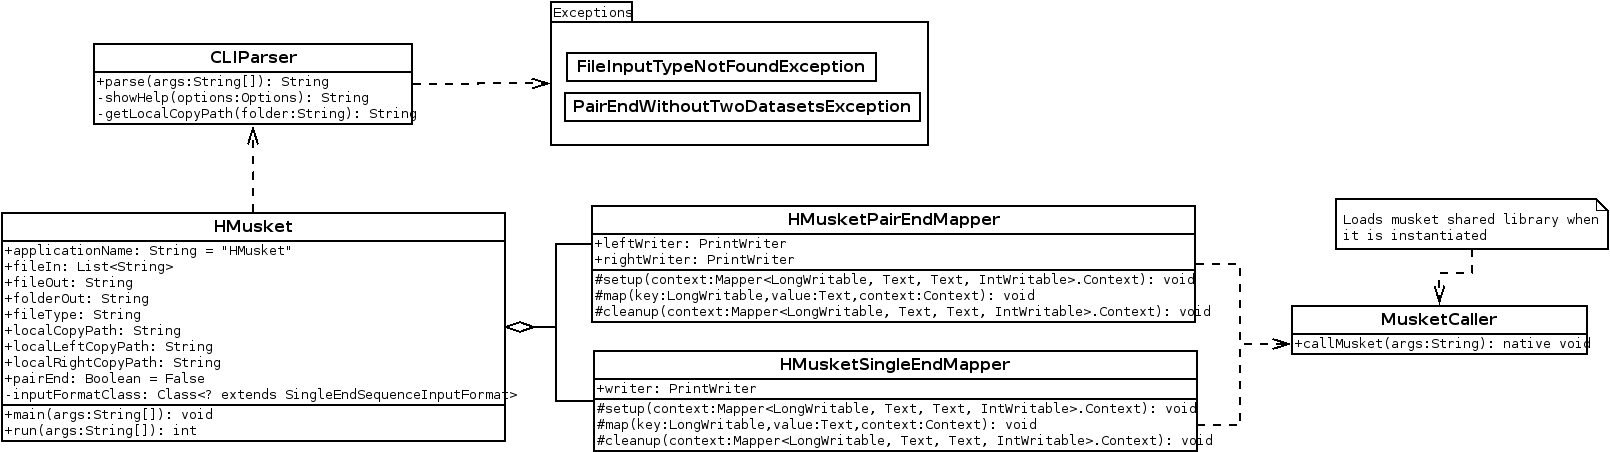
\includegraphics[width=20cm,height=5cm]{figures/hmusket.png}}
%	\caption{Diagrama de clases de HMusket}
%	\label{fig}
%\end{figure}

\subsection{Creación e integración de la librería}
Para poder realizar la llamada a código nativo lo primero de todo es convertir el software Musket en una shared library[*] para posteriormente instalarla en el cluster Hadoop y que de esta manera cualquier aplicación del ecosistema pueda hacer uso de la misma.\\
Para efectuar esta tarea lo primero de todo es crear una clase dentro del proyecto Java, en este caso fue en la clase MusketCaller, donde se especifique que durante la fase de instanciación cargue la librería nativa, en el caso del presente proyecto la librería ``musket''. Además de esta indicación se tiene que crear un método con la etiqueta ``native'', al igual que en los métodos abstractos tan solo se debe especificar la firma.\\
A continuación utilizando el comando ``javac'' se compila dicha clase generando un fichero .class, este fichero es requerido para generar el header file (.h), por medio del comando ``javah'' para posteriormente darle una implementación.\\
La implementación de ese header file se tiene que desarrollar un programa en C o C++ donde se incluya la cabecera generada en el paso anterior y la librería de JNI, implementar la firma indicada en el fichero de cabeceras y por último realizar la llamada de Musket.\\
Para poder realizar esta llamada como si fuera una librería en vez de un binario, se debe modificar el makefile del software en cuestión para añadir al compilador, en este caso el g++, los parámetros ``-fPIC'' y ``-shared''. Una vez compilada se añade al directorio \$HADOOP\_HOME/lib/native y por último se declarara la función main, del proyecto Musket, dentro del código C desarrollado.

\section{Evaluación experimental}
En primer lugar se detallará el entorno, tanto software como hardware, donde se realización las pruebas para que se puedan replicar los estudios y experimentos que se detallan a lo largo de esta sección. Posteriormente se indicara el estudio realizado sobre Musket para conocer la horquilla de tiempos a mejorar y los posibles cuellos de botella.\\
Para concluir, se expondrán los experimentos, resultados y conclusiones acerca de HMusket.

\subsection{Entorno de pruebas}
Para la realización de las diversas pruebas expuestas a lo largo de los siguientes párrafos se utilizó el cluster Plutón del Departamento de Ingeniería de Computadores, el cual consta con 18 nodos de cómputo de la siguientes características:\\ 

\begin{itemize}
	\item \textbf{CPU Model}: 2 × Intel Xeon E5-2660 Sandy Bridge-EP
	\item \textbf{CPU Speed/Turbo}: 2.20 GHz/3 GHz
	\item \textbf{Cores por CPU}: 8
	\item \textbf{Threads por core}: 2
	\item \textbf{Cores/Threads por nodo}: 16/32
	\item \textbf{Cache L1/L2/L3}: 32 KB/256 KB/20 MB
	\item \textbf{Memoria RAM}: 64 GB DDR3 1600 Mhz
	\item \textbf{Discos}: 1 × HDD 1 TB SATA3 7.2K rpm y 1 × SSD 480 GB SATA3 (de los nodos 8 a 15)
	\item \textbf{Redes}: InfiniBand FDR y Gigabit Ethernet\\
\end{itemize}

En resumen, el cluster cuenta con 1 nodo de login y 18 nodos de cómputo con un total de 288 cores físicos (576 threads) y 1.152 TB de memoria.\\

El sistema operativo que se ejecuta en estos servidores es Rocks 6.1[*] una distribución para entornos cluster basada en CentOS[*] 6.

\subsection{Análisis Musket}
Dado que Musket es un software acelerado mediante OpenMP (memoria compartida) el número máximo de threads con los que se pudo evaluar en el cluster fueron 16, y teniendo en cuenta que se requieren por lo menos 2 threads para funcionar (debido a patrón maestro/esclavo) se decidió evaluar el rendimiento de la aplicación con hilos de 2 a 16 en potencias de 2, es decir: 2, 4, 8, 16. Además se evaluaron dos dataset, uno con formato single-end de 49995929 secuencias de tamaño 100, y otro con formato pair-end (es decir, dos datasets) de 69247248 secuencias de tamaño 101 cada una, ambos de tipo Fastq y todo esto generando un espectro para k-mers de tamaño 2.\\

Tal y como se puede apreciar en la tabla 1 la paralelización de Musket presenta un carácter lineal pudiendo alcanzar un speed-up de aproximadamente 4.6977 para el dataset single-end y 8.6465 para el dataset pair-end. Resulta curioso, que siendo el dataset pair-end el doble de grande lo procese a en menos tiempo, esto puede ser debido a los k-mers que conforman el espectro del segundo dataset (pair-end) son menores y por lo tanto se repiten más que en el primer dataset, por tanto la evaluación de los mismos se efectúa de una manera más rápida.

%\begin{table}[]
%	\centering
%	\caption{Tabla experimental de Musket}
%	\label{tabla 1}
%	\begin{tabular}{|l|l|l|l|l|}
%		\hline
%		\textbf{Dataset} 	& \textbf{Threads} 	& \textbf{Number of sequence} & \textbf{Sequence size} & \textbf{Time} 				\\ \hline
%		Single-end 	& 2			& 49995929           & 100           & 13h: 29min: 21sec 	\\ \hline
%		Single-end 	& 4			& 49995929           & 100           & 08h: 44min: 17sec	\\ \hline
%		Single-end 	& 8			& 49995929           & 100           & 04h: 44min: 12sec 	\\ \hline
%		Single-end 	& 16		& 49995929           & 100           & 02h: 52min: 17sec 	\\ \hline \hline
%		Pair-end 	& 2			& 69247248           & 101           & 13h: 30min: 02sec 	\\ \hline
%		Pair-end 	& 4			& 69247248           & 101           & 04h: 30min: 15sec	\\ \hline
%		Pair-end 	& 8			& 69247248           & 101           & 02h: 24min: 34sec 	\\ \hline
%		Pair-end 	& 16		& 69247248           & 101           & 01h: 33min: 41sec 	\\ \hline
%	\end{tabular}
%\end{table}

\subsection{Análisis HMusket}
Para realizar las pruebas de HMusket se estudiaron y valoraron las posibles combinaciones de mapper por nodos que podían ser más eficientes a la hora de efectuar las funciones. Debido a que cada nodo se compone de 2 procesadores, de 8 núcleos cada uno, se estableció como máxima repartir en cada nodo a lo sumo 1 mapper por cada procesador, es decir, 1 o 2 mappers por cada nodo de computo. Esto implico que se tuviera que ajustar la memoria y el heap de los mappers (50Gb en caso de 1 mapper y 25Gb en caso de 2 mappers por nodo y en ambos casos se establece el 80\% de la memoria para el heap) por lo tanto, las combinaciones que se decidieron realizar para el experimento son los que se muestran en la tabla 2 junto con los resultados obtenidos en las diferentes pruebas.\\

Para la realización de pruebas en el cluster se utilizo BDEv[*], por medio de esta herramienta se puede desplegar un cluster Hadoop con todo su ecosistema de aplicaciones, pudiéndolo configurar de manera sencilla, simplemente hace falta terner una versión del JDK[*] en el entorno. Además de todo esto, BDEv provee de estadísticas e informes de evaluación acerca de como fue el rendimiento de la aplicación durante la ejecución.\\
No obstante el principal motivo para utilizar esta herramienta fue para poder ejecutar la aplicación distribuida en el sistema de colas del cluster, ya que de por si solo, el cluster no cuenta con el entorno Hadoop para los usuarios y actualmente no hay una solución para la integración este tipo de aplicaciones en los sistemas de colas.\\

%\begin{table}[]
%	\centering
%	\caption{Tabla experimental de HMusket}
%	\label{tabla 2}
%	\begin{tabular}{|l|l|l|l|l|l|l|l|l|}
%		\hline
%		\textbf{Dataset} &	\textbf{Number of nodes} & \textbf{Mapper/Node} & \textbf{Threads/Node} & \textbf{Memory/Mapper} & \textbf{Number of sequenc}e & \textbf{Sequence size} & \textbf{Time} & \textbf{Output merge time}	\\ \hline
%		Single-end &	4 & 1 & 16 & Memory/Mapper & Number of sequence & Sequence size & Time	& Output merge time	\\ \hline
%		Single-end &	4 & 2 & 8 & Memory/Mapper & Number of sequence & Sequence size & Time	& Output merge time	\\ \hline
%		Single-end &	8 & 1 & 16 & Memory/Mapper & Number of sequence & Sequence size & Time	& Output merge time	\\ \hline
%		Single-end &	8 & 2 & 8 & Memory/Mapper & Number of sequence & Sequence size & Time	& Output merge time	\\ \hline
%	\end{tabular}
%\end{table}

Dados los resultados obtenidos en los experimentos realizados on HMusket se puede concluir que el procesamiento que realiza esta herramienta sobre los conjuntos de datos de entrada escala de una manera linear, y que es mucho más eficiente repartir los 16 cores de un nodo entre dos mappers, de esta manera que se paraleliza mucho más el trabajo.\\

\section{Conclusiones y trabajo futuro}
Teniendo en cuenta todo lo indicando a lo largo de este artículo se puede concluir con que Musket es una herramienta bastante potente, de hecho de las mejores que hay actualmente, pero nos es capaz de hacer frente a la alta demanda de datos que ha surgido a lo largo de los últimos años.\\
Una buena alternativa para este problema es implementar o reutilizar ese software en un entorno de memoria distribuida, como por ejemplo Hadoop, mediante el paradigma Map/Reduce. Además, si se realiza una configuración adecuada se puede se puede mejorar el rendimiento de la aplicación en un x\%.\\

Como trabajo futuro sería interesante realizar ciertas modificaciones tanto el la librería Musket como en la aplicación distribuida para evitar las comunicaciones usando la entrada y salida estándar en lugar de ficheros y comparar el rendimiento de esta segunda versión frente a la aquí expuesta.

\section*{Referencias bibliográficas}
%
%Please number citations consecutively within brackets \cite{b1}. The 
%sentence punctuation follows the bracket \cite{b2}. Refer simply to the reference 
%number, as in \cite{b3}---do not use ``Ref. \cite{b3}'' or ``reference \cite{b3}'' except at 
%the beginning of a sentence: ``Reference \cite{b3} was the first $\ldots$''
%
%Number footnotes separately in superscripts. Place the actual footnote at 
%the bottom of the column in which it was cited. Do not put footnotes in the 
%abstract or reference list. Use letters for table footnotes.
%
%Unless there are six authors or more give all authors' names; do not use 
%``et al.''. Papers that have not been published, even if they have been 
%submitted for publication, should be cited as ``unpublished'' \cite{b4}. Papers 
%that have been accepted for publication should be cited as ``in press'' \cite{b5}. 
%Capitalize only the first word in a paper title, except for proper nouns and 
%element symbols.
%
%For papers published in translation journals, please give the English 
%citation first, followed by the original foreign-language citation \cite{b6}.
%
%\begin{thebibliography}{00}
%\bibitem{b1} G. Eason, B. Noble, and I. N. Sneddon, ``On certain integrals of Lipschitz-Hankel type involving products of Bessel functions,'' Phil. Trans. Roy. Soc. London, vol. A247, pp. 529--551, April 1955.
%\bibitem{b2} J. Clerk Maxwell, A Treatise on Electricity and Magnetism, 3rd ed., vol. 2. Oxford: Clarendon, 1892, pp.68--73.
%\bibitem{b3} I. S. Jacobs and C. P. Bean, ``Fine particles, thin films and exchange anisotropy,'' in Magnetism, vol. III, G. T. Rado and H. Suhl, Eds. New York: Academic, 1963, pp. 271--350.
%\bibitem{b4} K. Elissa, ``Title of paper if known,'' unpublished.
%\bibitem{b5} R. Nicole, ``Title of paper with only first word capitalized,'' J. Name Stand. Abbrev., in press.
%\bibitem{b6} Y. Yorozu, M. Hirano, K. Oka, and Y. Tagawa, ``Electron spectroscopy studies on magneto-optical media and plastic substrate interface,'' IEEE Transl. J. Magn. Japan, vol. 2, pp. 740--741, August 1987 [Digests 9th Annual Conf. Magnetics Japan, p. 301, 1982].
%\bibitem{b7} M. Young, The Technical Writer's Handbook. Mill Valley, CA: University Science, 1989.
%\end{thebibliography}

\end{document}
